% Created 2021-01-24 Sun 22:48
% Intended LaTeX compiler: pdflatex
\documentclass[11pt]{article}
\usepackage[utf8]{inputenc}
\usepackage[T1]{fontenc}
\usepackage{graphicx}
\usepackage{grffile}
\usepackage{longtable}
\usepackage{wrapfig}
\usepackage{rotating}
\usepackage[normalem]{ulem}
\usepackage{amsmath}
\usepackage{textcomp}
\usepackage{amssymb}
\usepackage{capt-of}
\usepackage{hyperref}
\usepackage{minted}
\hypersetup{colorlinks=true, linkcolor=black, filecolor=red, urlcolor=blue}
\usepackage[turkish]{babel}
\author{Eren Hatırnaz}
\date{29 Haziran 2020}
\title{Yazılım Gündemi - 2020/25\\\medskip
\large 22-28 Haziran 2020}
\hypersetup{
 pdfauthor={Eren Hatırnaz},
 pdftitle={Yazılım Gündemi - 2020/25},
 pdfkeywords={},
 pdfsubject={},
 pdfcreator={Emacs 27.1 (Org mode 9.3)},
 pdflang={Turkish}}
\begin{document}

\maketitle
\tableofcontents \clearpage\shorthandoff{=}

\begin{center}
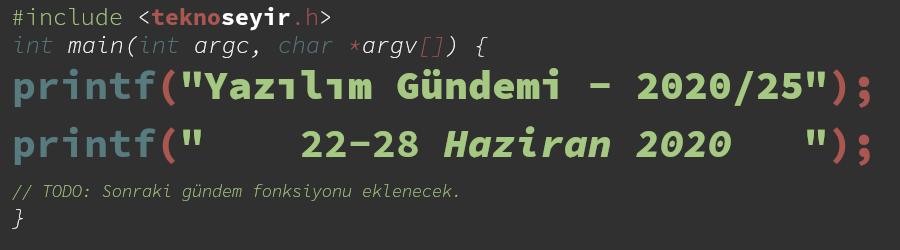
\includegraphics[width=.9\linewidth]{gorseller/yazilim-gundemi-banner.png}
\end{center}

\begin{center}
\href{../24/yazilim-gundemi-2020-24.pdf}{< Önceki Gündem} | \textbf{22-28 Haziran 2020} | \href{../26/yazilim-gundemi-2020-26.pdf}{Sonraki Gündem >}

\href{https://teknoseyir.com/blog/yazilim-gundemi-2020-25}{TeknoSeyir'de Oku}
\end{center}

\section{Container güvenliği ile ilgili gelişmeler: \href{https://blog.trendmicro.com/trendlabs-security-intelligence/xorddos-kaiji-botnet-malware-variants-target-exposed-docker-servers/}{XORDDoS}, \href{https://intezer.com/blog/research/kaiji-new-chinese-linux-malware-turning-to-golang/}{Kaiji} ve \href{https://unit42.paloaltonetworks.com/cryptojacking-docker-images-for-mining-monero/}{kripto para madenciliği}}
\label{sec:orgd7713ea}
Container teknolojisinin yaygınlaşmasıyla birlikte güvenlik sorunlarının da ön
plana çıktığını zaten yazılım gündemi yazılarında sürekli dile getiriyorum.
Geçtiğimiz hafta ise yine Container teknolojisini hedef alan birçok güvenlik
açığı ortaya çıkarıldı.

Bunlardan ilk ikisi Trend Micro güvenlik araştırmacıları tarafından ortaya
çıkarılan ve Docker sunucularını botnet ağına katarak DDoS saldırıları
gerçekleştirmeye yarayan XORDDoS (\href{https://www.trendmicro.com/vinfo/us/threat-encyclopedia/malware/Backdoor.Linux.XORDDOS.AE}{Backdoor.Linux.XORDDOS.AE}) ve Kaiji DDoS
(\href{https://www.trendmicro.com/vinfo/us/threat-encyclopedia/malware/DDoS.Linux.KAIJI.A}{DDoS.Linux.KAIJI.A}) isimli zararlılar. XORDDoS zararlısı sistemdeki tüm
Docker konteynerlerini tarayıp kendini onlara enjekte ederken diğeri Kaiji ise
kendi zararlı docker konteynerlerini oluşturup, onları çalıştırıyor.
Dolayısıyla Kaiji'yi tespit etmek daha kolay. Eğer \texttt{docker ps} komutunu
çalıştırdıktan sonra çıkan listede tanımadığımız bir konteyner varsa onlardan
şüphelenebilirsiniz.

Geçtiğimiz hafta içinde ortaya çıkan bir diğer olay ise, Docker Hub
platformundaki "azurenql" isimli kullanıcının paylaştığı Kripto para
madenciliği için kullanılan Docker İmaj'ları. Kullanıcı adını Microsoft'un
Azure bulut hizmetine benzetmiş ve bu sayede platforma yüklediği imajlar
yüzlerce kez indirilmiş.

\begin{figure}[htbp]
\centering
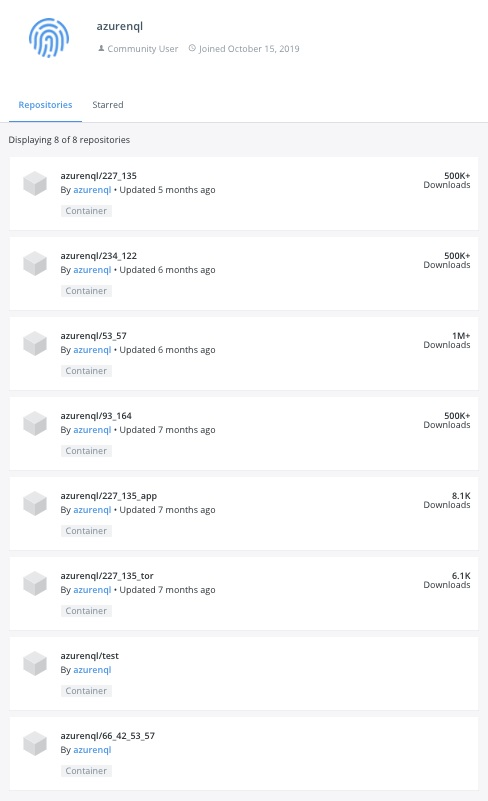
\includegraphics[height=12cm]{gorseller/docker-hub-azurenql.jpg}
\caption{"azurenql" isimli kullanıcının paylaştığı docker imajları}
\end{figure}

Paloalto Networks isimli firmanın altındaki Unit 42 güvenlik takımı bu
imajları ortaya çıkardıktan sonra hepsi silinmiş ve ilgili Docker Hub
kullanıcısı da sistemden atılmış. Fakat bu imajların yayınlandığı tarihten
(Ekim 2019) bu yana ilgili kripto para cüzdanı için 36.000\$'dan (525.38 XMR)
fazla para madencilik yoluyla oluşturulmuş. Yani yapan kişi bayağı bir para
kazanmış gözüküyor.

Bu haberdeki birçok güvenlik açığına yol açan sorun ise Docker'ı yönetmek için
kullanılan port numarasının (2375) tüm internete açılmış olması. Kötü amaçlı
kişiler interneti tarayarak bu açık portları yakalayıp, ilgili sistemlere
girebiliyor. Dolayısıyla yapılması gereken ilk iş bu portu internete kapatmak.
Daha sonra da sunucularınızda çalışan docker konteynerlerini kontrol etmek.
\section{Apple WWDC20 etkinliğinde duyurulan bazı gelişmeler}
\label{sec:org8a1c36c}
Apple, geçtiğimiz hafta Pazartesi günü World Wide Developers Conference 2020
(WWDC20) etkinliğini gerçekleştirdi. Her ne kadar isminde "geliştiriciler"
ifadesi geçse de Apple'ın daha çok son kullanıcılar için duyurular yaptığı bu
etkinliğe damgasını vuran konu ise Apple'ın Mac sistemlerde Intel
işlemcilerden kendi ARM tabanlı işlemcisine geçecek olması oldu. Daha çok son
kullanıcıları ilgilen konular için TeknoSeyir'de yayınlanan \href{https://teknoseyir.com/apple-wwdc20-degerlendirmesi}{Apple WWDC2
Değerlendirmesi} videosunu izleyebilirsiniz. Ben bu yazıda daha çok
geliştiricileri ilgilendiren bazı kısımlara değineceğim.

Öncelikle en baştan söylemek gerek ki Apple'ın bu ARM tabanlı kendi
işlemcisine geçme işi hemen gerçekleşecek bir şey değil (teknik olarak mümkün
olsa da pratikte sorunlar yaratır). Bu geçiş 2 yıllık bir süreçe yayılmış
durumda. Bu geçiş süreci elbette bağımsız geliştiricilerin uygulamalarını ARM
tabanına geçirmesini de içeriyor. Bu bağlamda Apple, geçtiğimiz hafta
içerisinde \href{https://developer.apple.com/programs/universal/}{Universal App Quick Start Program}'ını duyurdu.

\begin{figure}[htbp]
\centering
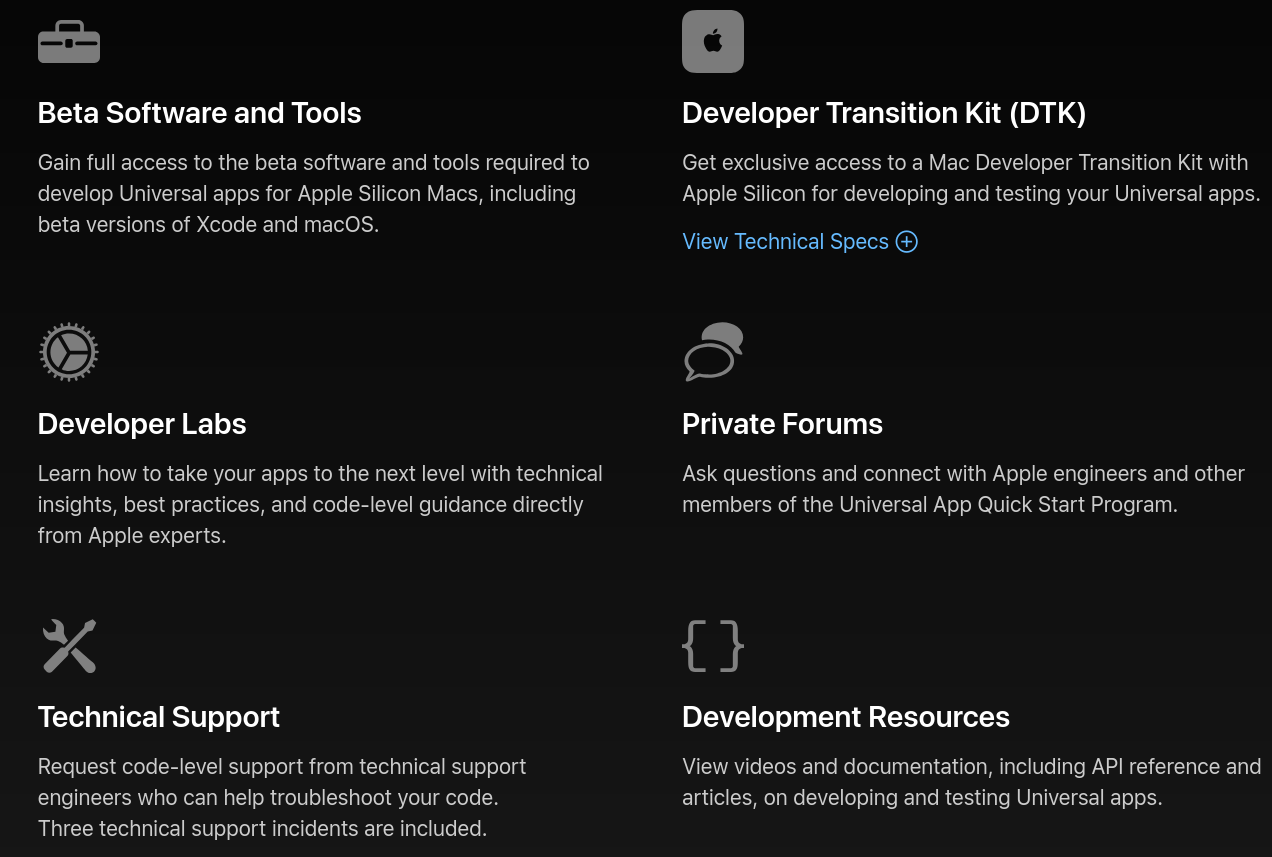
\includegraphics[height=5cm]{gorseller/apple-universal-app-quick-start-program.png}
\caption{Programın içeriği: Beta yazılım ve araçlara erişim, Geliştirici Geçiş Kiti (Donanım), Developer Labs, özel forumlar, teknik destek ve geliştirme için dokümantasyonlar}
\end{figure}

Yalnız bu programa başvurmak ücretsiz değil. Apple yukarıdaki hizmetler için
geliştiricilerden 500 Dolar talep ediyor ve henüz ülkemizden sipariş
edilemiyor. Donanımsal bir değişim olduğu için elbette Apple, bu programa
başvuran kişi ve firmalara ARM tabanlı, geliştirme için kullanılabilecek bir
kit sistemi de veriyor. Tabii ki program tamamlandığında geri verilmesi
kaydıyla.

Bu yılın sonunda ve 2021'in başında ilk ARM tabanlı ürünleri çıkarmaya
başlayacaklar fakat tabii ki bu süre zarfında tüm geliştiricilerin ARM
tabanına geçmesi mümkün değil. İşte bu sorunu çözmek adına Apple, geçmişte de
PowerPC'den Intel'e geçerken kullandığı Rosetta emülatörünü tekrar canlandırıp
Rosetta 2 ismiyle işletim sisteminin içine gömecek. Yüklediğiniz bir uygulama
eğer x86\_64 mimarisi komutlarını barındırıyorsa bu uygulama otomatik olarak
tanınacak ve Rosetta 2 emülatörü ile ARM tabanına dönüştürülüp,
çalıştırılacak. Native ARM tabanlı uygulama kadar performanslı olamayacağı
söylense de bunun zaten geçiş süreci içerisinde kullanılacak bir ara çözüm
olduğu düşünülünce pek sıkıntı çıkaracağını düşünmüyorum. Yalnız bunun da
birkaç kısıtlaması mevcut: JIT (Just-in-time) derleyicisi içeren uygulamalar,
Kernel eklentileri ve sanal makine uygulamalarını ARM tabanına dönüştüremiyor.
Bu da demek oluyor ki WMWare vb. yazılımların şu anki \href{https://www.macrumors.com/2020/06/23/rosetta-wont-support-x86-virtualization-windows/}{halleriyle orada
çalışamayacak}. Elbette ilgili firmalar ARM tabanlı sistemler için
sanallaştırma çözümlerini geliştireceklerdir ileriki zamanlarda.

Benim önüme düşen bir diğer yenilik ise iOS tarafında: \href{https://developer.apple.com/app-clips/}{App Clips}. Artık
kullanıcılarımıza uygulamamızın tamamını yüklemeden sadece küçük bir parçasını
kullandırabileceğiz. Bu küçük parça uygulama da işi bitince kullanıcıya
uygulamanın tam halini yüklemesi de tabii ki teklif ediliyor. Yani bir nevi
demo sunabileceğiniz kullanıcılara.

Apple'ın mobil cihazlarındaki uygulama marketinin işleyişiyle ilgili de bir
değişiklik söz konusu. Artık geliştiriciler App Store kurallarını \href{https://www.theverge.com/2020/6/22/21299814/apple-app-store-policies-ios-bug-fixes-approval-dispute-appeal}{ihlal ettiği
durumlarda Apple'a itiraz edebilecekler}. Apple da bu süre zarfında
kullanıcıların hatalardan mağdur olmaması için geliştiriciye hata giderme
güncellemelerini yayınlama izini verecek.

Konferansı canlı olarak izlemedim. Sadece takip ettiğim kaynaklardan önüme
düşen haberlere göz atıp değerlendirmelerimi yaptım. Haliyle duyurulan her
konuya yer verememiş olabilirim. Eğer bu konferansta duyurulan ve
geliştiricileri ilgilendiren başka konular biliyorsanız yorumlar bölümünde
dile getirebilirsiniz.
\section{GitLab \href{https://about.gitlab.com/releases/2020/06/22/gitlab-13-1-released/}{13.1 sürümü yayınlandı}}
\label{sec:org0b15588}
GitLab, geçtiğimiz hafta içerisinde 13.1 sürümünü yayınladı. Bu sürümden
gözüme çarpan bazı yenilik ve değişiklikler ise şu şekilde:

\subsection{\href{https://about.gitlab.com/releases/2020/06/22/gitlab-13-1-released/\#merge-request-reviews-moved-to-core}{Merge Request Reviews artık herkese açık}}
\label{sec:org38c70d9}
\begin{center}
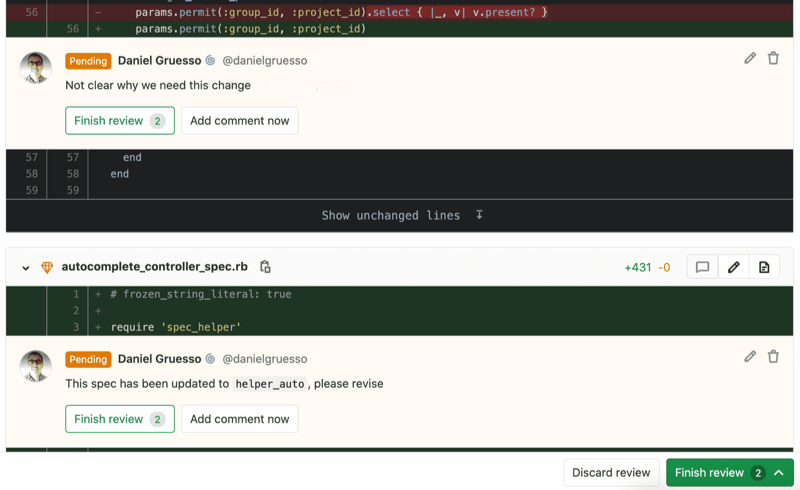
\includegraphics[width=.9\linewidth]{gorseller/gitlab-merge-request-reviews.png}
\end{center}

İlk olarak GitLab 11.4 sürümüyle birlikte GitLab Premium özelliği olarak
sunulan bu özellik artık herkesin kullanımına açıldı. Artık bir merge
request'i review ederken birden çok yorumu tek seferde yazıp
gönderebileceksiniz. Böylece karşı tarafın e-posta kutusu da birden çok
maille dolmamış olacak.
\subsection{\href{https://about.gitlab.com/releases/2020/06/22/gitlab-13-1-released/\#run-tests-for-modified-files-first}{Değiştirilen dosyalar için testleri önceliklendirme}}
\label{sec:org137bee5}
Büyük projelerde kod yazarken en can sıkıcı şeylerden biri de kodunuzu uzak
git sunucusuna gönderdiğiniz çalışan CI/CD süreçlerinin sonuçlanmasını
beklemek. Bazen yeni yazdığınız bir testin geçemediğiniz görmeniz için çok
uzun süreler beklemeniz gerekebiliyor. İşte GitLab da tam bu soruna çözüm
getirmiş ve eğer bir test dosyasında değişiklik yapılmışsa o dosyadaki
testleri daha önce çalıştırıyor ve sonuçlarını gösteriyor. Böylece vakit
kazanmış oluyorsunuz. Yalnız bu özellik henüz ücretsiz sürümde mevcut değil.
\subsection{\href{https://about.gitlab.com/releases/2020/06/22/gitlab-13-1-released/\#code-intelligence}{Code Intelligence}}
\label{sec:org9f68aa6}
\begin{center}
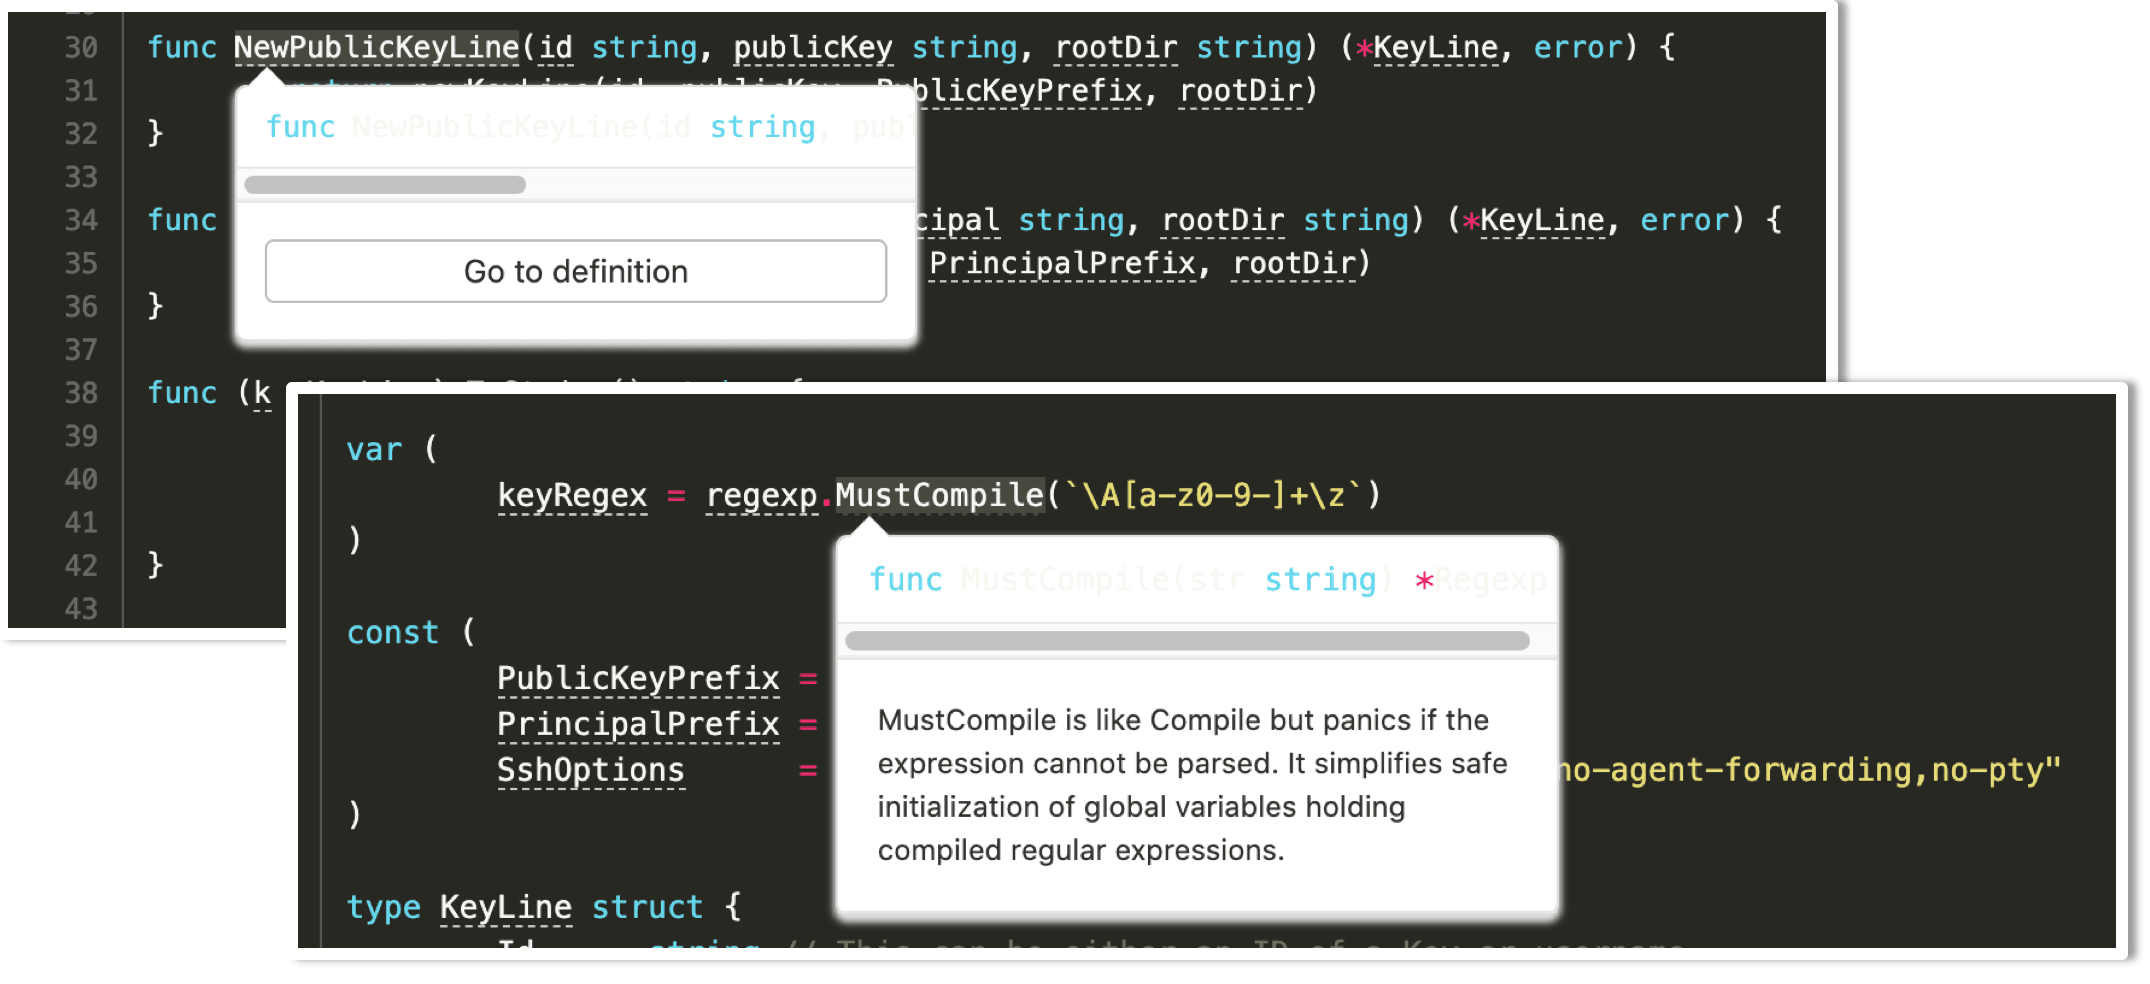
\includegraphics[width=.9\linewidth]{gorseller/gitlab-code-intelligence.png}
\end{center}

GitLab ve Sourcegraph partnerliğiyle ortaya çıkan bu özellikle birlikte artık
GitLab'ın Web IDE'sinde kodlarda gezinirken bir fonksiyonun üzerine
geldiğimizde onun dokümantasyon bilgilerini görebileceğiz ve istersek
tanımlandığı dosyayı açabileceğiz. Ayrıca bu sürümle birlikte Web IDE'ye
EditorConfig \href{https://about.gitlab.com/releases/2020/06/22/gitlab-13-1-released/\#code-intelligence}{desteği de gelmiş}. Bugüne kadar olmaması şaşırttı beni.

İlgili sürüm notları sayfası epeyce bir uzun hepsine göz atamadım fakat
baktıklarım ve GitLab'ın kendi öne çıkardıkları içerisinde gözüme çarpanları
aktarmak istedim. Diğer gelişmeler ve değişiklikler için konu başlığına
eklediğim bağlantıya tıklayabilirsiniz.
\section{GitHub ana sayfa ve depo sayfalarının tasarımını \href{https://github.blog/changelog/2020-06-23-design-updates-to-repositories-and-github-ui/}{güncelledi}}
\label{sec:org0eda56c}
Aslında bir önceki gündem yazısında değerlendirecektim bu konuyu ama GitHub
ile ilgili iki tane önemli gelişme verken bir GitHub haberi daha eklemek hem
çeşitliliği azaltacaktı hem de bir hafta önce bu değişiklik henüz beta
aşamasındaydı. Bu hafta ise artık beta'dan çıkmış ve resmi olarak duyurulmuş
durumda.

\begin{figure}[htbp]
\centering
\includegraphics[width=.9\linewidth]{gorseller/github-yeni-tasarım.png}
\caption{GitHub'ın yeni depo sayfası tasarımı.}
\end{figure}

Görülebildiği gibi profil resimleri dahil tüm elemanlara kenar yuvarlatma
işlemi uygulanmış. Ayrıca ikonlar da değiştirilmiş. Benim henüz alışamadığım
bir değişiklik de eskiden üst kısımda olan kısa depo açıklaması, versiyon
bilgileri, kullanılan programlama dilleri gibi görselliklerin sağ tarafa
taşınmış olması oldu. Bir depo sayfasına girdiğimde istemsiz olarak ilk üst
kısma bakıyorum, bulamayınca yana bakıyorum. Buna alışabilirim bir süre sonra
ama hâlâ daha karanlık tema özelliğinin gelmemiş olmasına ne alışabiliyorum,
ne de tahammül edemiyorum. Gerçekten anlamakta zorlanıyorum. Geliştiriciler
için hazırlanmamış birçok sitede bile bu özellik varken GitHub gibi çoğunlukla
bizim kullandığımız ve geceleri aktif olduğumuz bir platformun karanlık tema
özelliğin olmaması nereden bakarsanız bakın saçmalıktır! Beta süresindeyken
geri bildirim olarak göndermiştim fakat dikkate alınmamış demek ki. GitHub'dan
biraz soğumaya başladım ne yalan söyleyeyim.

Yeni tasarım hakkında siz ne düşünüyorsunuz? Alışabildiniz mi yoksa siz de
benim gibi elemanların eski tasarımdaki yerlerine hala bakanlardan mısınız?
Karanlık temasının hala daha gelmemiş olmasına kaç rezalet puanı verirsiniz?
Yorumlar bölümünde konuşalım.
\section{Python'a Pattern Matching özelliği eklenmesi için \href{https://www.python.org/dev/peps/pep-0622/}{taslak öneri sunuldu}}
\label{sec:org33a919c}
Geçtiğimiz hafta içerisinde yayınlanan taslak öneri dokümanıyla birlikte eğer
öneri kabul edilirse artık Python'da şu bir söz dizimi (syntax) yazmak mümkün
olacak:

\newpage
\begin{minted}[breaklines=true,breakanywhere=true,frame=lines, label=Python]{python}
match degisken:
    case 0 | 1 | 2:
        print("Küçük sayı")
    case [] | [_]:
        print("Kısa bir dizi")
    case str():
        print("String bir ifade")
    case _:
        print("Başka bir şeyler")
\end{minted}

Türkçe'ye örüntü tanıma ya da desen tanıma olarak çevirirsek yanlış olmaz
sanırım. Bu özellikle birlikte gördüğünüz gibi birden çok sorgulama ifadesini
tek bir değişken için çalıştırabileceğiz. Python'da diğer birçok dilde olan
switch/case yapısının olmaması da düşünüldüğünde bence böyle bir özelliğe
günümüzde ihtiyaç var.

Daha önce de bir tane dilin yaratıcısı tarafından olmak üzere 2 kez denenmiş
bu özelliğin eklenmesi fakat kabul edilmemiş (bkz: \href{https://www.python.org/dev/peps/pep-0275/}{PEP 275}) (bkz: \href{https://www.python.org/dev/peps/pep-3103/}{PEP 3103}).
Bakalım bu seferki denemenin sonucu ne olacak? Hep birlikte göreceğiz.
\section{Angular \href{https://blog.angular.io/version-10-of-angular-now-available-78960babd41}{10.0.0 sürümü yayınlandı}}
\label{sec:org179058b}
Eskilerin popüler ön yüz geliştirme frameworklerinden biri olan Angular
geliştirilmeye devam ediyor. Geçtiğimiz hafta yayınlanan 10.0.0 sürümüyle
birlikte gelen bazı özellik ve değişiklikler ise şu şekilde:

\url{gorseller/angular10-date-range-picker.gif}

Yeni Date Range Picker elemanını \texttt{mat-date-range-input} ve
\texttt{mat-date-range-picker} komponentleriyle birlikte kullanabilirsiniz. Daha
fazla detay için \href{https://next.material.angular.io/components/datepicker/overview\#date-range-selection}{bu sayfayı ziyaret edebilirsiniz}.

Ayrıca bu sürümle birlikte opsiyonel olarak "strict" mod özelliği de gelmiş
durumda. Yeni bir proje oluştururken \texttt{ng new -{}-strict} komutunu kullanırsanız
bu modun aktif olduğu bir proje yaratabilirsiniz.

Angular'ın geliştirilmesi için kullanılan teknolojilerin sürümleri
de yükseltilmiş. Bunlar arasında TypeScript 3.9 sürümüne geçiş, TSLib ve
TSLint araçlarının güncellenmesi de var.

Bu sürümle birlikte gelen diğer özellik ve değişiklikler için konu başlığına
eklediğim bağlantıya tıklayabilirsiniz. Eğer projenizi Angular 10 sürümüne
yükseltmek istiyorsanız yükseltme rehberi için bu sayfayı ziyaret
edebilirsiniz: \url{https://update.angular.io/}.
\section{Perl \href{https://www.perl.com/article/announcing-perl-7/}{7 sürümü duyuruldu}}
\label{sec:orgbaa4a03}
Geçtiğimiz hafta düzenlenen Perl konferansında, Perl programlama dilinin yeni
sürümü olan Perl 7 duyuruldu. Fakat düşündüğünüz gibi büyük kod değişiklikleri
içeren bir sürüm değil, daha çok Perl 5'in daha modern varsayılan ayarlarla
birlikte gelen hali gibi düşünebilirsiniz. Tabii ki ileride büyük kod
değişiklikleri içeren major sürümler de gelecek.

\href{https://www.youtube.com/watch?v=6wPMh-3qYJM}{Konuyla ilgili YouTube videosu}

Bu aynı zamanda demek oluyor ki Perl 6 sürümü hiçbir zaman olmayacak. Bana PHP
5'den PHP 7'ye geçişi hatırlattı bu durum. İlginç bir bilgi: PHP 6 etiketli
bir sürüm olmamasına rağmen Türkiye'de bir yayınevi bu isimde kitap basmıştır
:).
\section{Yaklaşan Online Etkinlikler}
\label{sec:orgbe1f3b6}
\begin{longtable}{|p{9.5cm}|l|}
\hline
Etkinlik İsmi & Tarihi\\
\hline
\endfirsthead
\multicolumn{2}{l}{Önceki sayfadan devam ediyor} \\
\hline

Etkinlik İsmi & Tarihi \\

\hline
\endhead
\hline\multicolumn{2}{r}{Devamı sonraki sayfada} \\
\endfoot
\endlastfoot
\hline
\href{https://kommunity.com/pgtr/events/postgresql-sohbetleri-25-veri-tipleri-ileri-seviye-b80d6bfc}{PostgreSQL Sohbetleri 25: Veri tipleri (ileri seviye)} & 29 Haziran 13:30\\
\href{https://www.meetup.com/tr-TR/IBMDeveloperTR/events/270949858/}{Build a ML model for calculating product order return propensity} & 29 Haziran 14:00\\
\href{https://www.meetup.com/tr-TR/IBMDeveloperTR/events/270785212/}{Serverless Uygulamalarınızı OpenShift'te Operatörlerle Yönetin!} & 29 Haziran 15:00\\
\href{https://www.meetup.com/tr-TR/FirebaseTR/events/270991062/}{How to use Firestore?} & 29 Haziran 21:00\\
\href{https://www.meetup.com/tr-TR/Microsoft-Giri\%25C5\%259Fimcilik-Bulu\%25C5\%259Fmalar\%25C4\%25B1/events/271443638/}{Cloud Native MySQL \& PostgreSQL in Azure: The Future of Open Source Databases} & 30 Haziran 13:00\\
\href{https://www.meetup.com/tr-TR/Cloud-Computing-Technologists/events/270604890/}{AWS Public Sector Summit Online} & 30 Haziran 16:00\\
\href{https://www.meetup.com/tr-TR/IBMDeveloperTR/events/270949795/}{Predict your insurance premium cost with AutoAI} & 30 Haziran 18:00\\
\href{https://www.meetup.com/tr-TR/Istanbul-Java-User-Group/events/271377159/}{Hem Kazan Hem Öğren :: Tasarım Kalıpları Part-2} & 30 Haziran 19:00\\
\href{https://www.meetup.com/tr-TR/python-istanbul/events/271526409/}{Python Saati no.115-Dinamik Programlama ile Antik Yazılar Üzerinde Çalışmak} & 30 Haziran 20:00\\
\href{https://www.meetup.com/tr-TR/GDG-Hatay/events/270946487/}{What's New in Android 11} & 30 Haziran 20:00\\
\href{https://kommunity.com/acmhacettepe/events/nodejs-deno-ve-js-ile-backend-gelistirmenin-dunu-ve-bugunu-eser-ozvataf-5ef2730a}{Eser Özvataf - Node.js, Deno ve JS ile Backend Geliştirmenin Dünü ve Bugünü} & 30 Haziran 21:00\\
\href{https://kommunity.com/tracikkaynak/events/online-yarisma-turkce-dogal-dil-isleme-4e93a5ba}{Online Yarışma: Türkçe Doğal Dil İşleme} & 1 Temmuz 09:00\\
\href{https://www.meetup.com/tr-TR/IBMDeveloperTR/events/271308690/}{Uydu datalarını Watson Studio ile analiz etme} & 1 Temmuz 15:00\\
\href{https://www.meetup.com/tr-TR/Oracle-Developer-Meetup-Istanbul/events/271414254/}{Managed Kubernetes - firing up a full cluster \& deploying \& running apps on K8S} & 1 Temmuz 18:00\\
\href{https://www.meetup.com/tr-TR/IBMDeveloperTR/events/271471757/}{OpenShift Pipelines 101: Journey to Save Time} & 2 Temmuz 14:00\\
\href{https://kommunity.com/mobilerdev/events/fluttera-dogru-7-webview-ile-uygulama-olusturmak-cb0ebe4e}{Flutter'a Doğru no.7 - Webview ile Uygulama Oluşturmak} & 2 Temmuz 21:00\\
\href{https://www.meetup.com/tr-TR/IBMDeveloperTR/events/271471860/}{Build your First Microservice based Web Application} & 3 Temmuz 14:00\\
\href{https://kommunity.com/devnot-yazilimci-bulusmalari/events/custom-distributed-transaction-management-between-microservices-850b0f3c}{Custom Distributed Transaction Management Between Microservices} & 3 Temmuz 21:00\\
\href{https://www.meetup.com/tr-TR/IBMDeveloperTR/events/271471941/}{Create a web-based chatbot with voice input and output} & 4 Temmuz 14:00\\
\hline
\end{longtable}
\section{Diğer Haberler}
\label{sec:orgc64e240}
\begin{itemize}
\item İngiltere Ulusal Siber Güvenlik Merkezi: "\href{https://www.ncsc.gov.uk/blog-post/let-them-paste-passwords}{Parola yapıştırmaya izin verin}"
\item Unity Learn Premium \href{https://blogs.unity3d.com/2020/06/23/learn-premium-is-now-available-to-everyone-at-no-cost-forever/}{herkes için ücretsiz oldu}.
\item AWS, kod yazmadan uygulama geliştirme \href{https://aws.amazon.com/tr/blogs/aws/introducing-amazon-honeycode-build-web-mobile-apps-without-writing-code/}{çözümünü beta olarak tanıttı}: \href{https://www.honeycode.aws}{Amazon
Honeycode}.
\item HashiCorp Cloud Platform \href{https://www.hashicorp.com/blog/announcing-cloud-platform/}{tanıtıldı}.
\item Snapchat geliştiriciler için ücretsiz telefon doğrulama \href{https://techcrunch.com/2020/06/23/snapchat-adds-free-phone-number-verification-to-its-list-of-sdk-perks/}{hizmetini tanıttı}.
\item GitHub Enterpise Server \href{https://github.blog/2020-06-25-github-enterprise-server-2-21-is-here/}{2.21 sürümü yayınlandı}.
\item dotnet-monitor \href{https://devblogs.microsoft.com/dotnet/introducing-dotnet-monitor/}{projesi tanıtıldı}.
\item Windows 10 ARM için \href{https://devblogs.microsoft.com/java/announcing-openjdk-windows-arm/}{OpenJDK duyuruldu}.
\item PHPStorm \href{https://blog.jetbrains.com/phpstorm/2020/06/phpstorm-2020-1-3-preview/}{2020.1.3 Preview sürümü yayınlandı}.
\item PHP \href{https://www.php.net/archive/2020.php\#2020-06-25-1}{8.0.0 Alpha 1 sürümü yayınlandı}.
\item TypeScript \href{https://devblogs.microsoft.com/typescript/announcing-typescript-4-0-beta/}{4.0 Beta sürümü yayınlandı}.
\item Flutter takımı, geliştiriciler için \href{https://medium.com/flutter/new-tools-for-flutter-developers-built-in-flutter-a122cb4eec86}{yeni araçlar yayınladılar}.
\item Deno \href{https://github.com/denoland/deno/releases/tag/v1.1.2}{v1.1.2 sürümü yayınlandı}.
\item Hasura Cloud \href{https://hasura.io/blog/announcing-hasura-cloud-managed-graphql-for-your-database-and-services/}{tanıtıldı}.
\item Haskell için web geliştirme framewürk'ü \href{https://ihp.digitallyinduced.com/}{tanıtıldı}: \href{https://github.com/digitallyinduced/ihp}{IHP}. \href{https://www.youtube.com/watch?v=UbDtS\_mUMpI\&feature=emb\_title}{YouTube Tanıtım
Videosu}
\item OneDev \href{https://www.onedev.io/v3.2.0/}{3.2 sürümü yayınlandı}.
\item Micronaut \href{https://objectcomputing.com/news/2020/06/26/announcing-micronaut-20}{2.0 sürümü yayınlandı}.
\item SQLDelight \href{https://github.com/cashapp/sqldelight/releases/tag/1.4.0}{1.4.0 sürümü yayınlandı}.
\item DVC \href{https://dvc.org/blog/dvc-1-0-release}{1.0 sürümü yayınlandı}.
\end{itemize}
\section{Lisans}
\label{sec:org8dc6922}
\begin{center}
\begin{center}

\includegraphics[height=1.5cm]{../../../img/CC_BY-NC-SA_4.0.png}
\end{center}

\href{yazilim-gundemi-2020-25.pdf}{Yazılım Gündemi - 2020/25} yazısı \href{https://erenhatirnaz.github.io}{Eren Hatırnaz} tarafından \href{http://creativecommons.org/licenses/by-nc-sa/4.0/}{Creative Commons
Atıf-GayriTicari-AynıLisanslaPaylaş 4.0 Uluslararası Lisansı} (CC BY-NC-SA 4.0)
ile lisanslanmıştır.
\end{center}
\end{document}
